\documentclass[10pt]{article}
\usepackage[polish]{babel}
\usepackage[utf8]{inputenc}
\usepackage[T1]{fontenc}
\usepackage{amsmath}
\usepackage{amsfonts}
\usepackage{amssymb}
\usepackage[version=4]{mhchem}
\usepackage{stmaryrd}
\usepackage{graphicx}
\usepackage[export]{adjustbox}
\graphicspath{ {./images/} }

\title{KLASY PIERWSZE I DRUGIE }

\author{}
\date{}


\begin{document}
\maketitle
\begin{enumerate}
  \item Operacją nazwiemy przyporządkowanie trójce liczb \((a, b, c)\) nowej trójki liczb \((b+c, c+a, a+b)\). Po wykonaniu 2023 takich operacji na otrzymywanych trójkach liczb, startując od trójki \((1,3,5)\) otrzymano \((x, y, z)\). Ile wynosi różnica \(x-y\) ?
  \item Na każdej ścianie sześcianu napisano pewną dodatnią liczbę całkowitą. Następnie w każdym wierzchołku sześcianu umieszczono liczbę, która jest równa iloczynowi liczb znajdujących się na ścianach, do których ten wierzchołek należy. Oblicz sumę liczb znajdujących się na wszystkich ścianach, wiedząc, że suma liczb umieszczonych w wierzchołkach wynosi 70.
  \item Punkty W, A, B, C są położone na płaszczyźnie tak, jak na rysunku obok (punkty A, B, C są współliniowe, kąt WAC jest prosty). Z punktów A, B i C widać wierzchołek wieży, której podstawa znajduje się w punkcie W odpowiednio pod kątami \(60^{\circ}, 45^{\circ}, 30^{\circ}\). Wykaż, że \(A B=B C\).\\
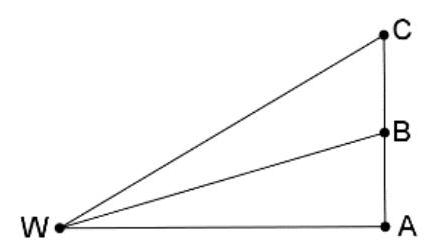
\includegraphics[max width=\textwidth, center]{2024_11_21_5f24e24876ae7b240204g-1}
\end{enumerate}

\section*{KLASY TRZECIE I CZWARTE}
\begin{enumerate}
  \item Dany jest trójkąt \(A B C\) o polu równym 1, w którym długości boków spełniają nierówności: \(a \geq b \geq c\). Udowodnij, że \(b \geq \sqrt{2}\).
  \item W trójkącie \(A B C C D\) jest dwusieczną. Udowodnij, że \(C D^{2}=a b\left(1-\frac{c^{2}}{(a+b)^{2}}\right)\).
  \item Czworokąt ABCD wpisany jest w okrąg. Na tym okręgu leży punkt P. Udowodnij, że iloczyn odległości punktu P od prostych \(A B\) i CD jest równy iloczynowi odległości punktu P od prostych BC i DA.
\end{enumerate}

\end{document}